47. \begin{figure}[ht!]
\center{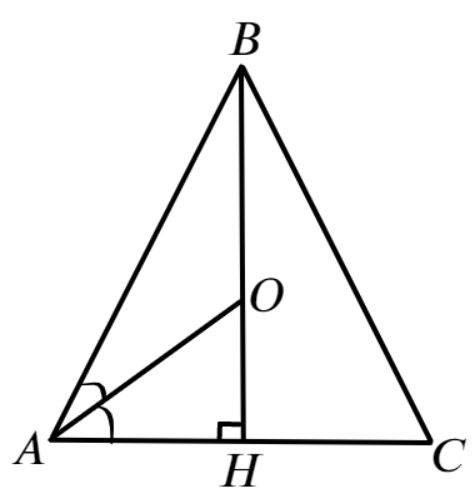
\includegraphics[scale=0.35]{g9-47.png}}
\end{figure}\\
Центр вписанного круга --- это точка пересечения биссектрис треугольника, значит делить он может только высоту, опущенную из вершины (совпадающую с биссектрисой). По свойству основания биссектрисы имеем соотношение $\cfrac{AB}{AH}=\cfrac{BO}{OH}.$ Возможны два случая: $\cfrac{60}{AH}=\cfrac{12}{5},\ AH=25,\ AC=50$см или
$\cfrac{60}{AH}=\cfrac{5}{12},\ AH=144,\ AC=288$см.\\
